% Intended LaTeX compiler: pdflatex
\documentclass[letterpaper, 12pt]{report}
\usepackage[utf8]{inputenc}
\usepackage[T1]{fontenc}
\usepackage{graphicx}
\usepackage{longtable}
\usepackage{wrapfig}
\usepackage{rotating}
\usepackage[normalem]{ulem}
\usepackage{amsmath}
\usepackage{amssymb}
\usepackage{capt-of}
\usepackage{hyperref}
\usepackage{amsmath}		% Extra math definitions
\usepackage{graphics}		% PostScript figures
\usepackage{setspace}		% 1.5 spacing
\usepackage{longtable}          % Tables spanning pages
\usepackage{natbib}
\usepackage{times}
\usepackage{url}
\usepackage{latexsym}
\usepackage[usenames]{color}
\usepackage{covington}
\usepackage{graphicx}
\usepackage{multirow}
\usepackage{subcaption}%#+LATEX_HEADER: \usepackage{subfigure}
\usepackage{booktabs}
\usepackage{tabularx}
\usepackage[T1]{fontenc}
\usepackage[utf8]{inputenc}
\usepackage[english]{babel}
\usepackage{blindtext}
\usepackage{amsfonts}
\usepackage{amsthm}
\usepackage[table,xcdraw]{xcolor}
\usepackage{rotating}
\usepackage{listings}
\definecolor{NiceBlue}{RGB}{11, 102, 163}
\definecolor{SlightRed}{RGB}{249,38,114}
\usepackage{textcomp} % other glyphs needed for upquote in listings below
\lstdefinelanguage{DemoExample}
{ basicstyle=\footnotesize \ttfamily,
commentstyle=\color{SlightRed} \rmfamily\itshape,
stringstyle=\color{NiceBlue},
morecomment=[s]{/*}{*/},
morestring=[b]'
}
\usepackage[fancyhdr]{macros/McECEThesis}	% Thesis style
\usepackage{McGillLogo}		% McGill University crest
\usepackage{color}
\insidemargin = 1.1in
\outsidemargin = 1.1in
\abovemargin = 1.1in
\belowmargin = 0.75in
\newcommand{\beq}{\begin{equation}}
\newcommand{\eeq}{\end{equation}}
\usepackage{palatino}           % Less abusive fonts
\usepackage{macros/palatcm}
\usepackage{hyperref}
\let\mathexp=\exp %redefine \exp to \mathexp cuz gb4e package redefines \exp
\usepackage{gb4e}
\noautomath
\usepackage[acronym,toc,section=section]{glossaries}

\makeglossaries

% GLossary entries
\newglossaryentry{tlm}{name=Transformers,description={{A class of models first derived by Vaswani et al. 2017}}}
% Acronyms
\newacronym{llm}{LLMs}{Large Language Models}
\newacronym{qos}{QoS}{quality-of-service}
\newacronym{bb}{BB}{branch and bound}


\author{Koustuv Sinha}
\date{}
\title{PhD Thesis}
\hypersetup{
 pdfauthor={Koustuv Sinha},
 pdftitle={PhD Thesis},
 pdfkeywords={},
 pdfsubject={},
 pdfcreator={Emacs 28.1 (Org mode 9.6)}, 
 pdflang={English}}
\begin{document}

\maketitle
\raggedbottom
\spacing{1.5}%\onehalfspacing
\pagenumbering{roman}

\chapter*{Acknowledgements}
\label{sec:org111920c}
\chapter*{Abstract}
\label{sec:orgec62e8c}
\chapter*{Abstract in French}
\label{sec:org71795cd}
\chapter*{Contributions to Original Knowledge}
\label{sec:org3bc5b8a}
\chapter*{Contributions of Authors}
\label{sec:org2435b5a}
\listoffigures{}

\chapter*{List of Tables}
\label{sec:org85f7663}
\clearpage
\setcounter{tocdepth}{3}
\tableofcontents

\clearpage

\pagenumbering{arabic}

\chapter{Introduction}
\label{sec:orgeb32902}

\textbf{\textbf{Central Theme of the thesis}} : Understanding systematicity in pre-trained language models through semantic and syntactic generalization.

In this thesis I discuss my work on understanding systematicity in pre-trained language models.

\clearpage

\chapter{Background}
\label{sec:orgaa03e11}

\section{Early methods for text representation}
\label{sec:org7176877}
\section{Neural Inductive bias of text representation}
\label{sec:org2479903}
\subsection{Feed Forward Neural Networks}
\label{sec:orgc5c64b1}
\subsection{Recurrent Neural Networks}
\label{sec:org081fc19}
\subsection{Transformer Models}
\label{sec:orgce0ee81}

\gls{llm} are the state-of-the-art in language models, which are based on \gls{tlm}.
\section{Pre-training and the advent of Large Language Models}
\label{sec:org754bcf3}
Success of pre-training and scale
\section{Systematicity and Generalization}
\label{sec:orgb799e4e}
\subsection{Definitions}
\label{sec:org70d8bf6}
\begin{enumerate}
\item Productivity
\label{sec:orgbb21691}
\item Word Order Sensitivity
\label{sec:org41a33eb}
\end{enumerate}
\subsection{Tasks}
\label{sec:org51f5f2f}
\clearpage
\chapter{Understanding semantic generalization through productivity}
\label{sec:org63ce972}

Natural language understanding (NLU) systems have been extremely successful at reading comprehension tasks, such as question answering (QA) and natural language inference (NLI).
An array of existing datasets are available for these tasks. This includes datasets that test a system's ability to extract factual answers from text \cite{Rajpurkar2016-yc,Nguyen2016-ec,Trischler2016-fc,Mostafazadeh2016-hu,Su2016-so}, as well as datasets that emphasize commonsense inference, such as entailment between sentences \cite{bowman2015large,williams2018broad}.

However, there are growing concerns regarding the ability of NLU systems---and neural networks more generally---to generalize in a systematic and robust way \cite{bahdanau2018systematic,lake2017generalization,Johnson2016-mw}.
For instance, recent work has highlighted the brittleness of NLU systems to adversarial examples \cite{jia2017adversarial}, as well as the fact that NLU models tend to exploit statistical artifacts in datasets, rather than exhibiting true reasoning and generalization capabilities \cite{gururangan2018annotation,kaushik2018much}.
These findings have also dovetailed with the recent dominance of large pre-trained language models, such as BERT, on NLU benchmarks \cite{devlin2018bert,peters2018deep}, which suggest that the primary difficulty in these datasets is incorporating the statistics of the natural language, rather than reasoning.

An important challenge is thus to develop NLU benchmarks that can precisely test a model's capability for robust and systematic generalization.
Ideally, we want language understanding systems that can not only answer questions and draw inferences from text, but that can also do so in a systematic, logical, and robust way.
While such reasoning capabilities are certainly required for many existing NLU tasks, most datasets combine several challenges of language understanding into one, such as co-reference/entity resolution, incorporating world knowledge, and semantic parsing---making it difficult to isolate and diagnose a model's capabilities for systematic generalization and robustness.

Inspired by the classic AI challenge of inductive logic programming \cite{Quinlan1990-iv}, in this chapter I discuss my work on developing semi-synthetic benchmark designed to explicitly test an NLU model's ability for systematic and robust logical generalization \cite{sinha2019a}.
Our benchmark suite---termed CLUTRR (Compositional Language Understanding and Text-based Relational Reasoning)---contains a large set of semi-synthetic stories involving hypothetical families.
Given a story, the goal is to infer the relationship between two family members, whose relationship is not explicitly mentioned.
To solve this task, a learning agent must extract the relationships mentioned in the text, induce the logical rules governing the kinship relationships (e.g., the transitivity of the sibling relation), and use these rules to infer the relationship between a given pair of entities.
Crucially, the CLUTRR benchmark allows us to test a learning agent's ability for \emph{systematic generalization} by testing on stories that contain unseen combinations of logical rules.
CLUTRR also allows us to precisely test for the various forms of \emph{model robustness} by adding different kinds of superfluous \emph{noise facts} to the stories.


\section{Technical Background}
\label{sec:org11db5fd}
\section{CLUTRR: A Diagnostic Benchmark for Inductive Reasoning in Text}
\label{sec:orgf6fb520}

Paper: \cite{sinha2019a}

\subsection{Dataset construction}
\label{sec:org086eed1}

\begin{figure}[htbp]
\centering
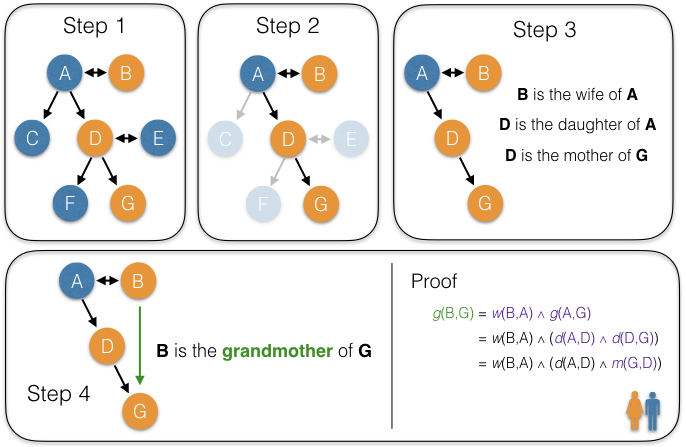
\includegraphics[height=0.3\textwidth]{figs/clutrr/dataset_const_proof.png}
\caption{Dataset generation pipeline.}
\end{figure}

\begin{figure}[htbp]
\centering
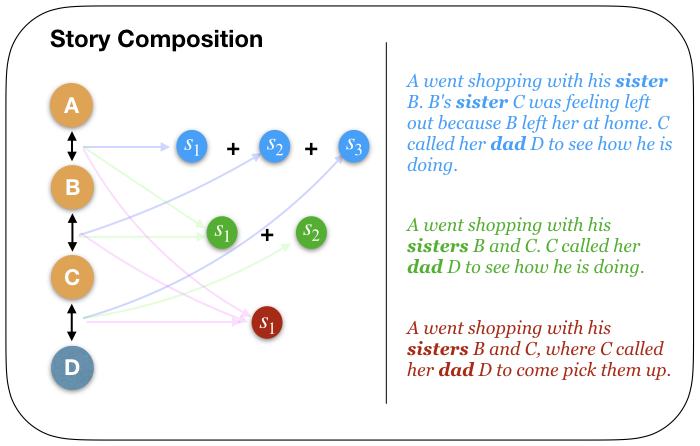
\includegraphics[height=0.3\textwidth]{figs/clutrr/composition.png}
\caption{Illustration of how a set of facts can split and combined in various ways across sentences.}
\end{figure}

\begin{figure}[htbp]
\centering
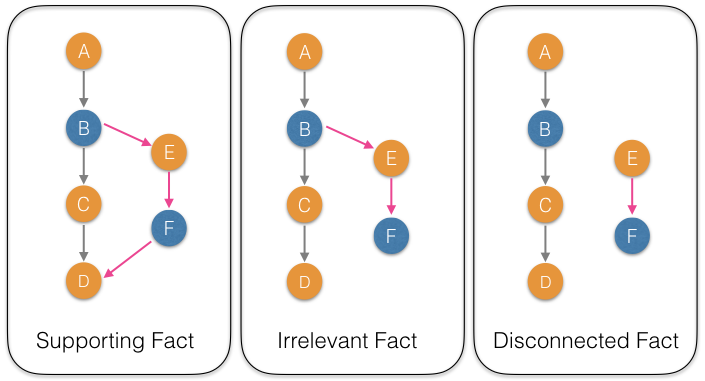
\includegraphics[height=0.3\textwidth]{figs/clutrr/clutrr_noise.png}
\caption{Noise generation procedures of CLUTRR.}
\end{figure}

\subsection{Productivity and reasoning}
\label{sec:orgcfb448d}
\section{Results}
\label{sec:org9950ca0}

\begin{center}
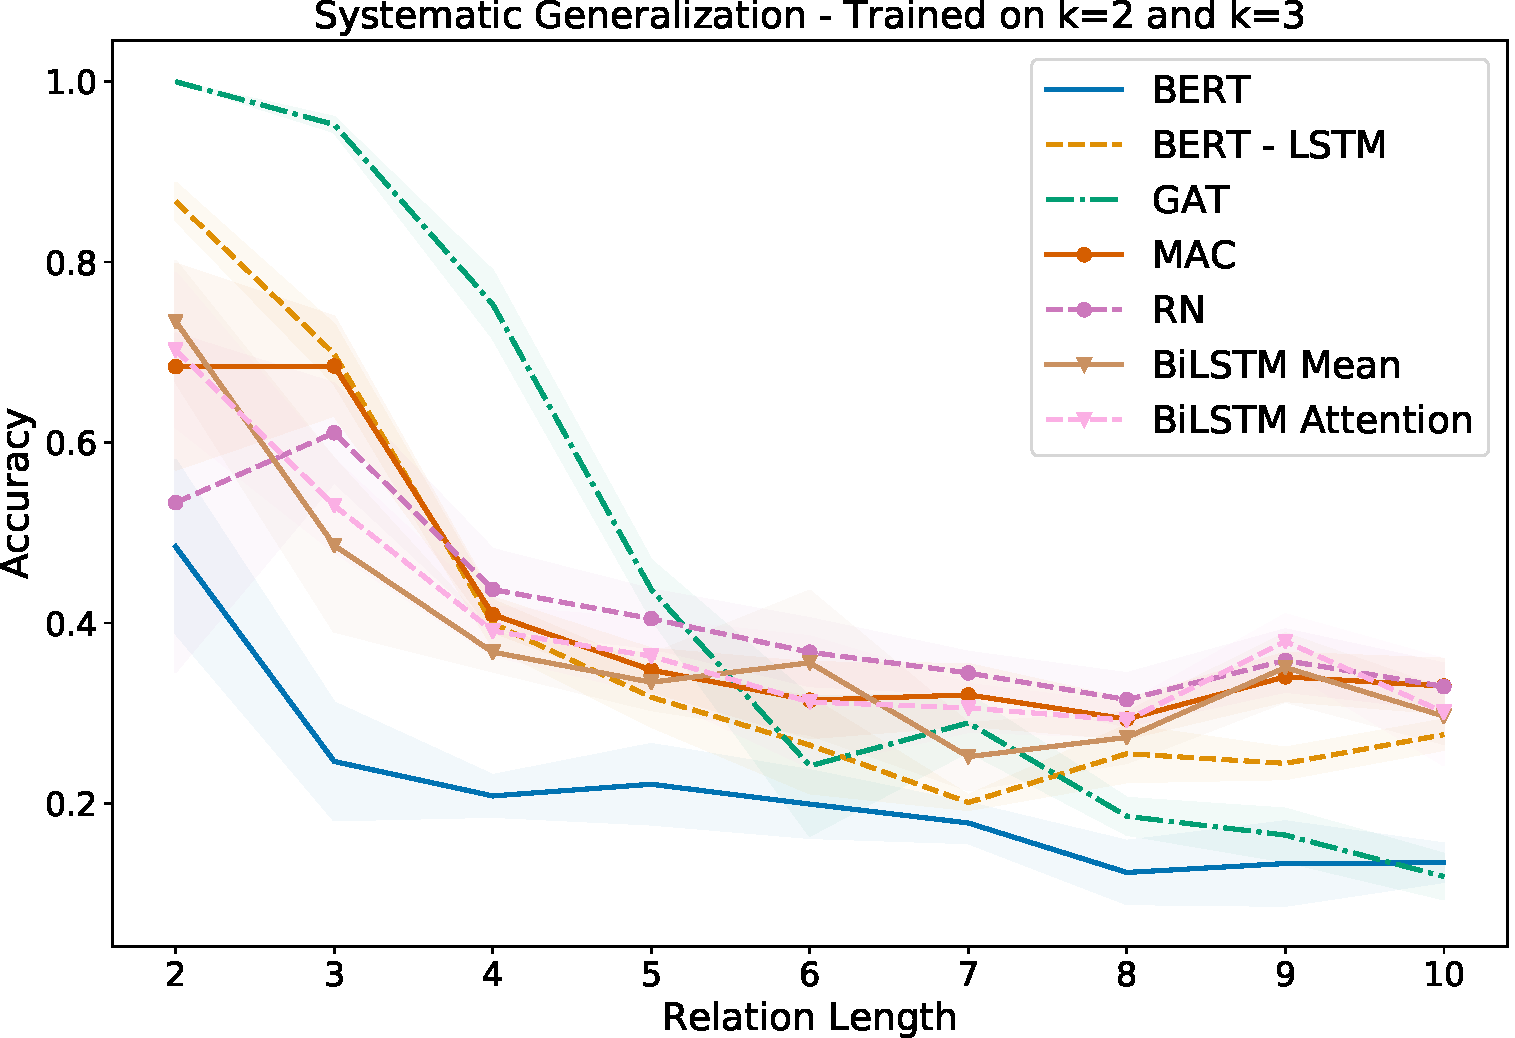
\includegraphics[height=0.3\textwidth]{figs/clutrr/emnlp/sys_gen_23.pdf}
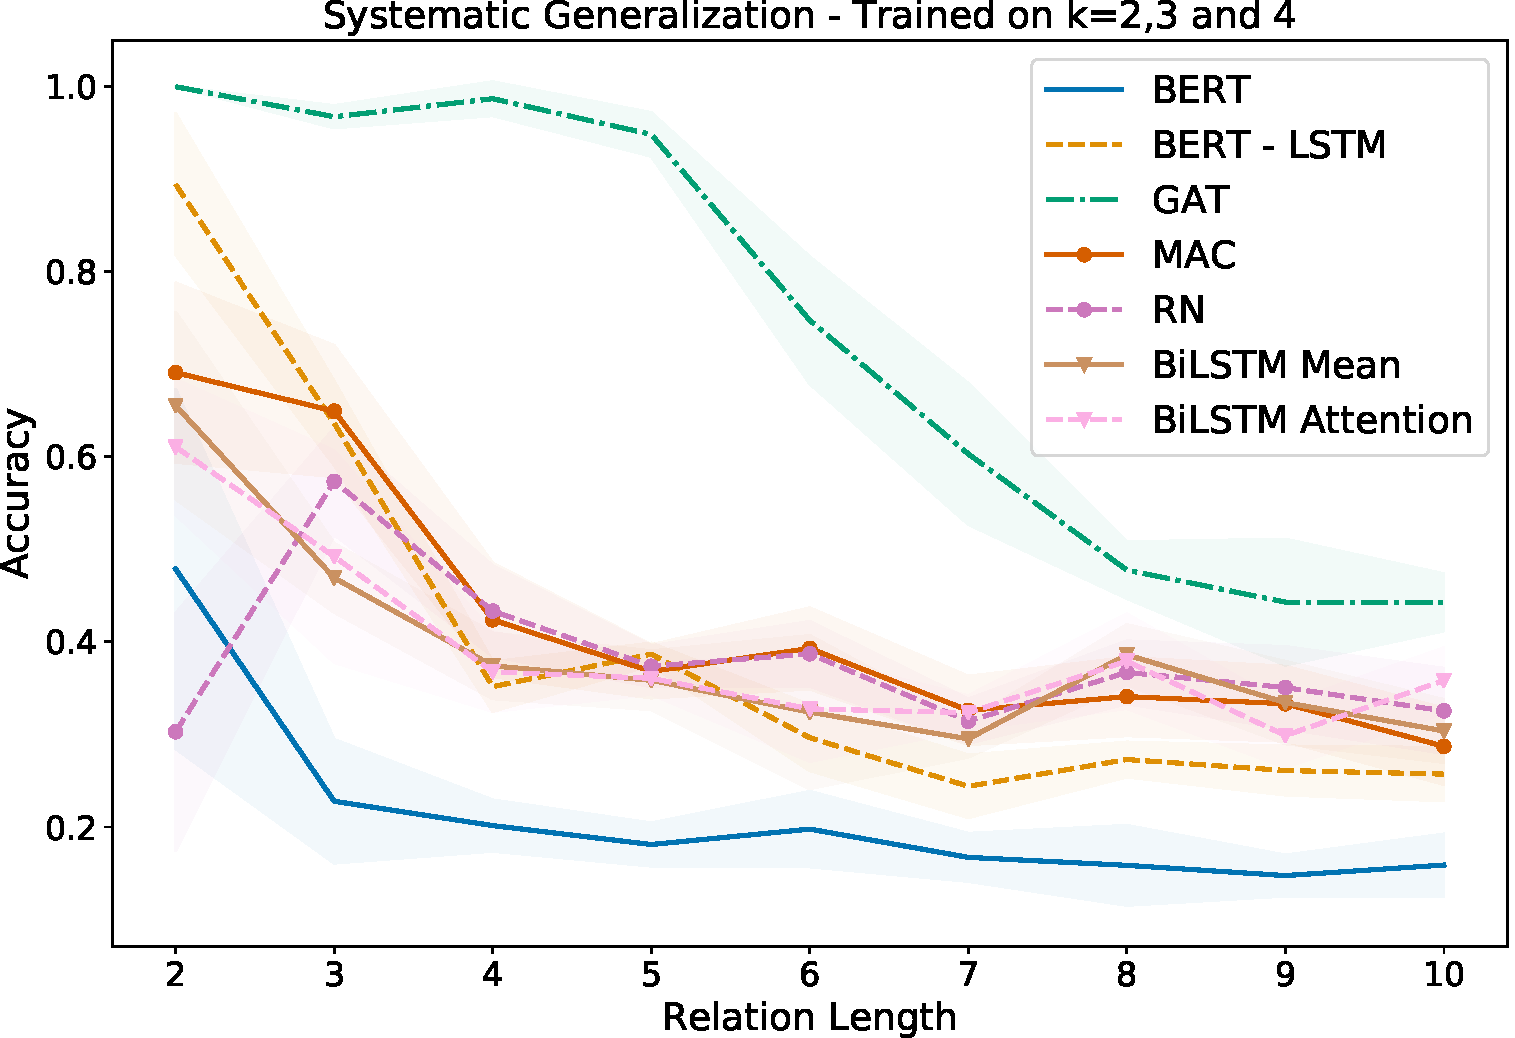
\includegraphics[height=0.3\textwidth]{figs/clutrr/emnlp/sys_gen_234.pdf}
\end{center}
\begin{figure}[htbp]
\centering

\includegraphics[height=0.0001in]{figs/empy_fig.png}
\caption{Systematic generalization when train on k=\(2\) and \(3\).}
\end{figure}


\section{Related Work}
\label{sec:org90fb063}
\section{Discussion}
\label{sec:orgaf96b9b}
\section{Follow-up findings in the community}
\label{sec:org53c3914}
\clearpage
\chapter{Quantifying syntactic generalization using word order}
\label{sec:orgc518e9d}

Paper \cite{sinha2021a}

\section{Technical Background}
\label{sec:org79bc56d}
\section{Word Order in Natural Language Inference}
\label{sec:org08e7337}
\subsection{Probe Construction}
\label{sec:orgaf44630}

\begin{figure}[htbp]
\centering
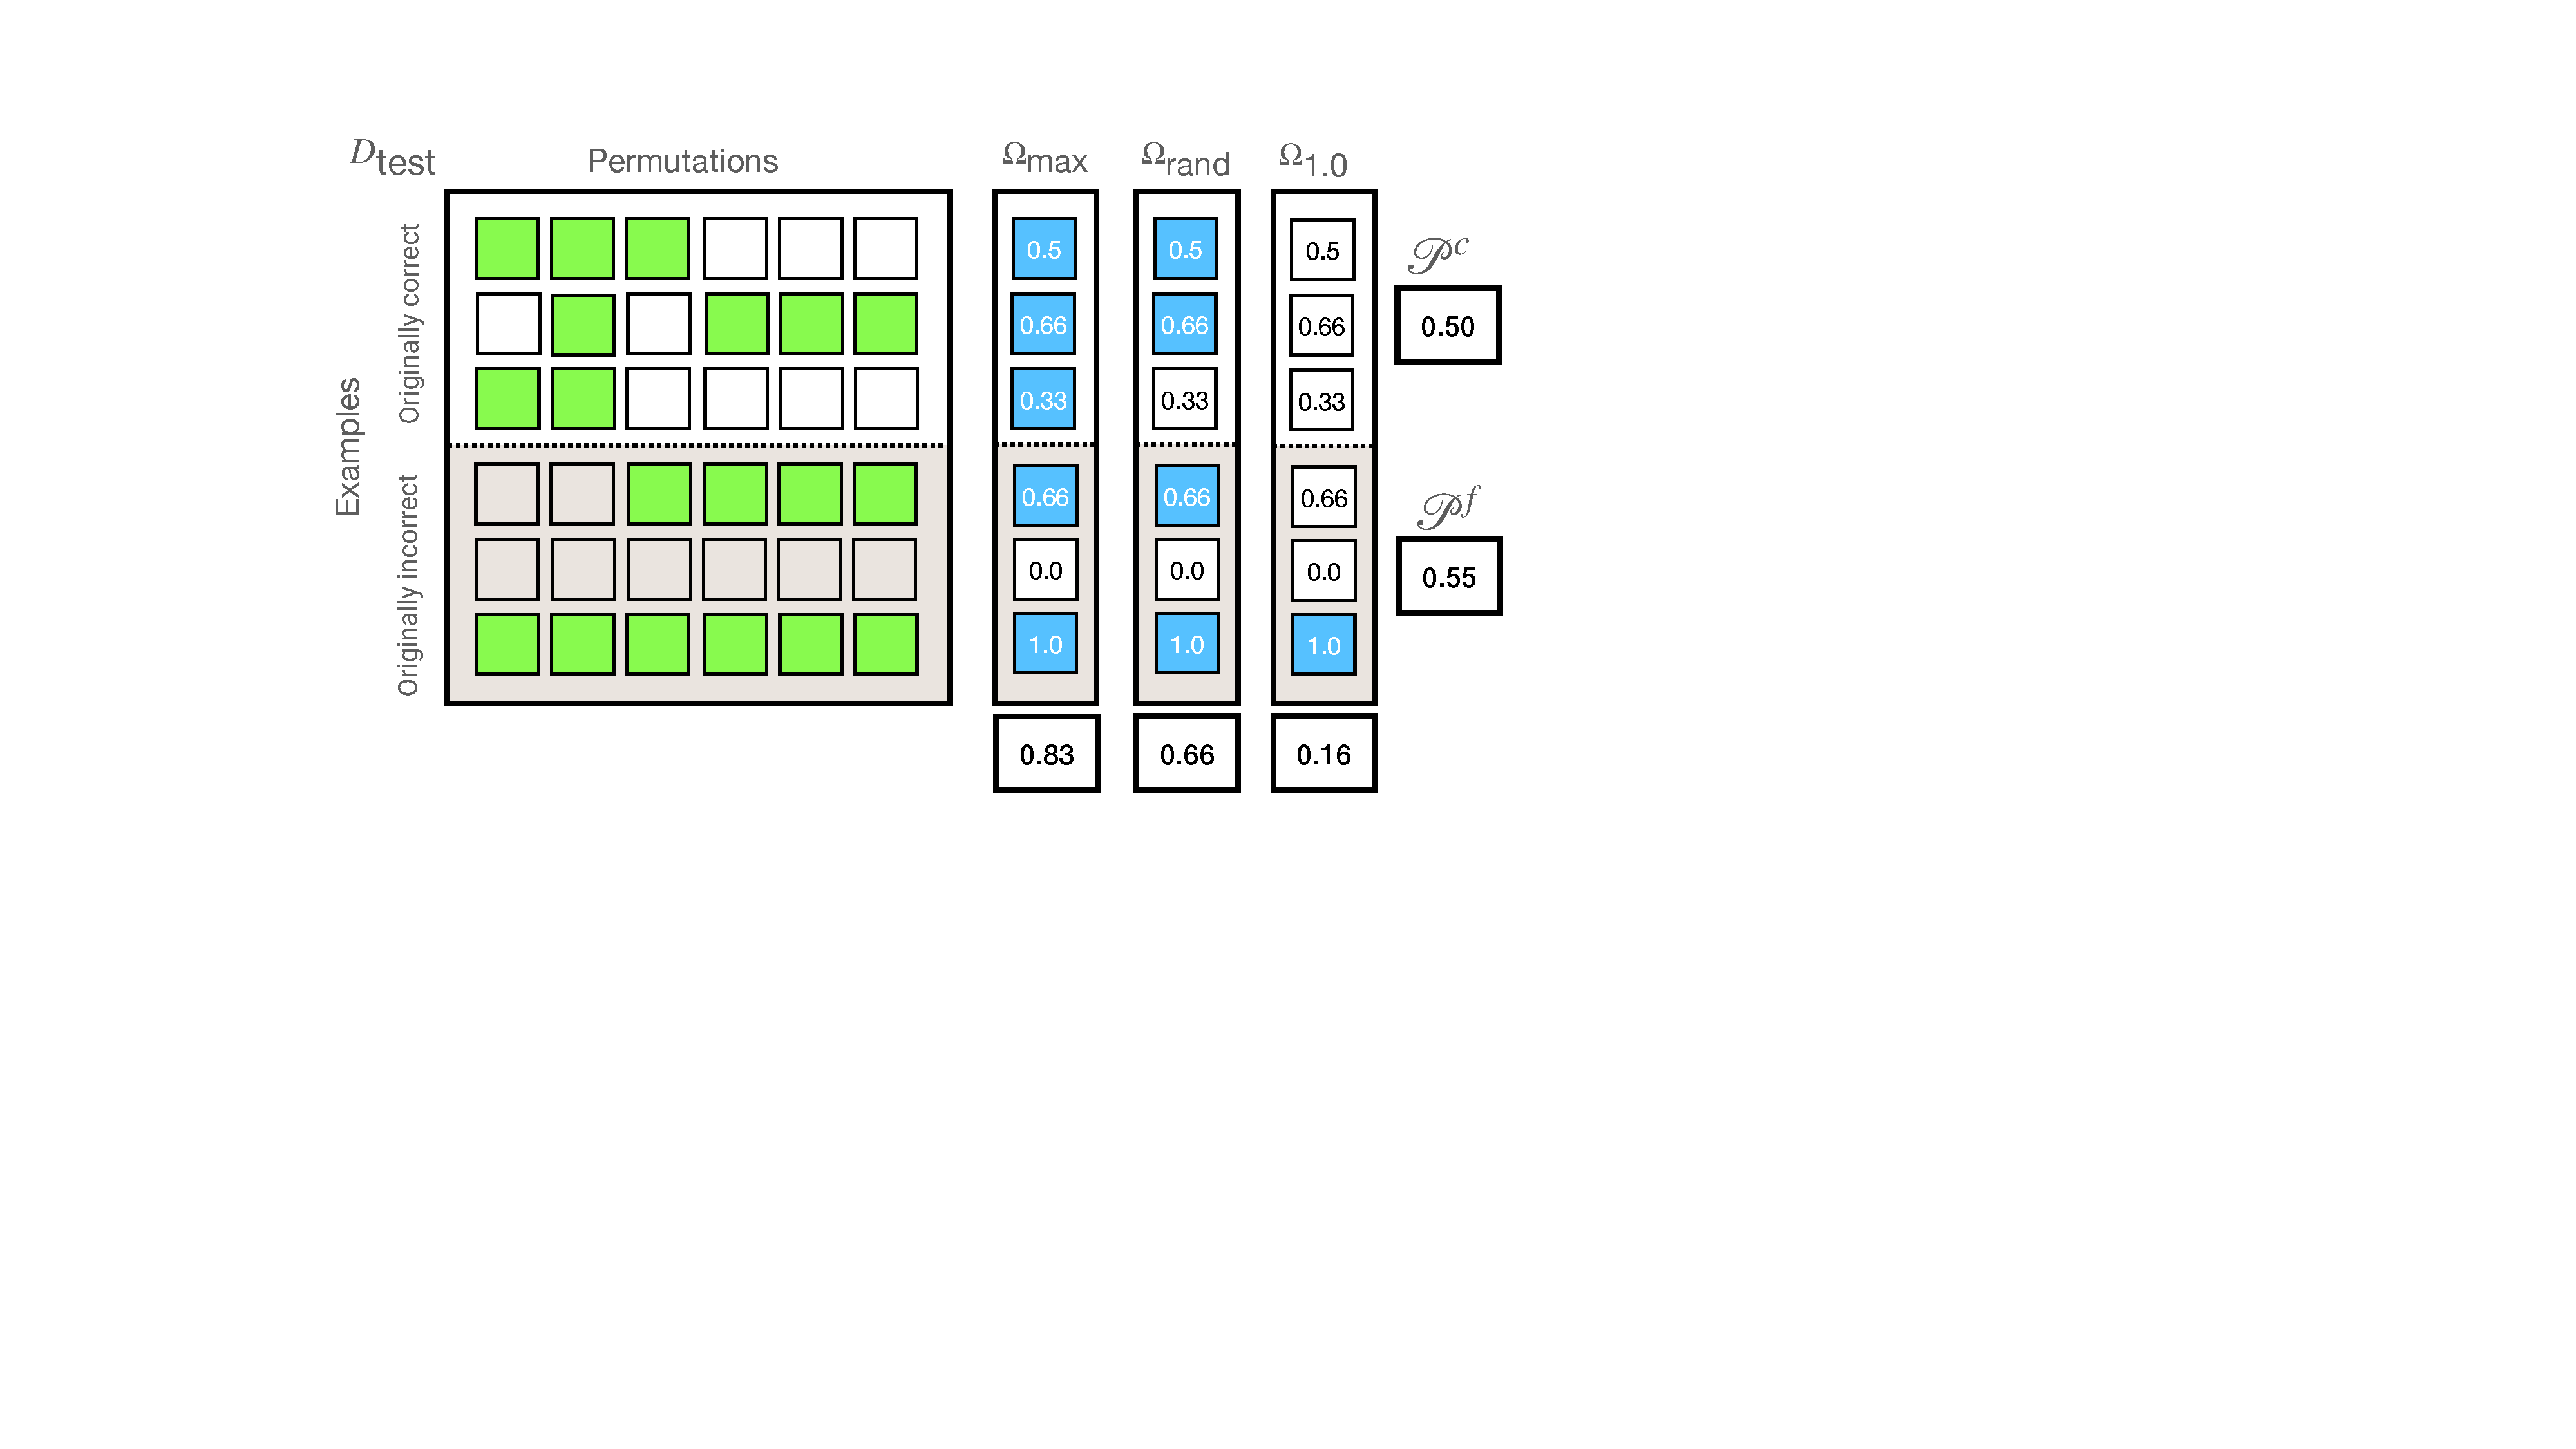
\includegraphics[height=0.3\textwidth]{figs/unli/nli_gen_perm_desc.pdf}
\caption{Graphical representation of the Permutation Acceptance class of metrics.}
\end{figure}

\section{Experiments \& Results}
\label{sec:org8b435b7}

\begin{figure}[htbp]
\centering
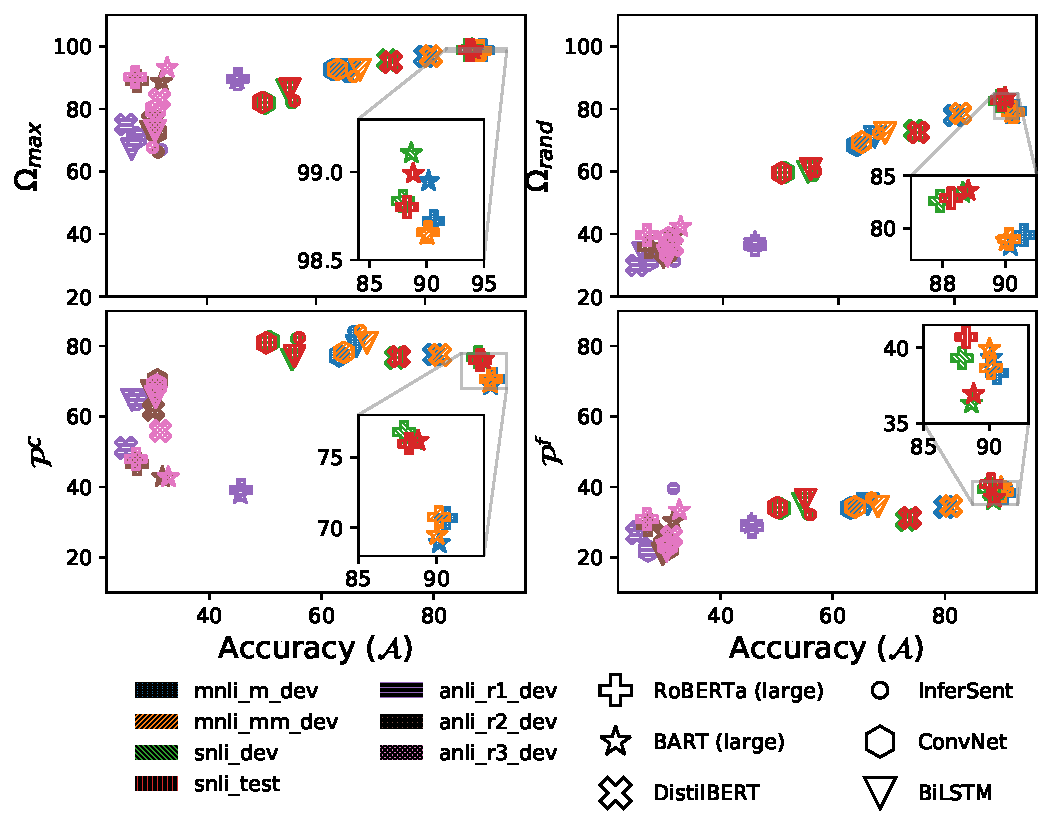
\includegraphics[width=.9\linewidth]{figs/unli/comb_plot_all.pdf}
\caption{Comparison of \(\omega_{\text{max}}\), \(\omega_{\text{rand}}\), \(\mathcal{P}^{c}\) and \(\mathcal{P}^{f}\) with the model accuracy \(\mathcal{A}\) on multiple datasets, where all models are trained on the MNLI corpus \cite{williams-etal-2018-broad}.}
\end{figure}

\begin{figure}[htbp]
\centering
\includegraphics[width=.9\linewidth]{figs/unli/all_entropy.png}
\caption{Average entropy of model confidences on permutations..}
\end{figure}

\begin{figure}[htbp]
\centering
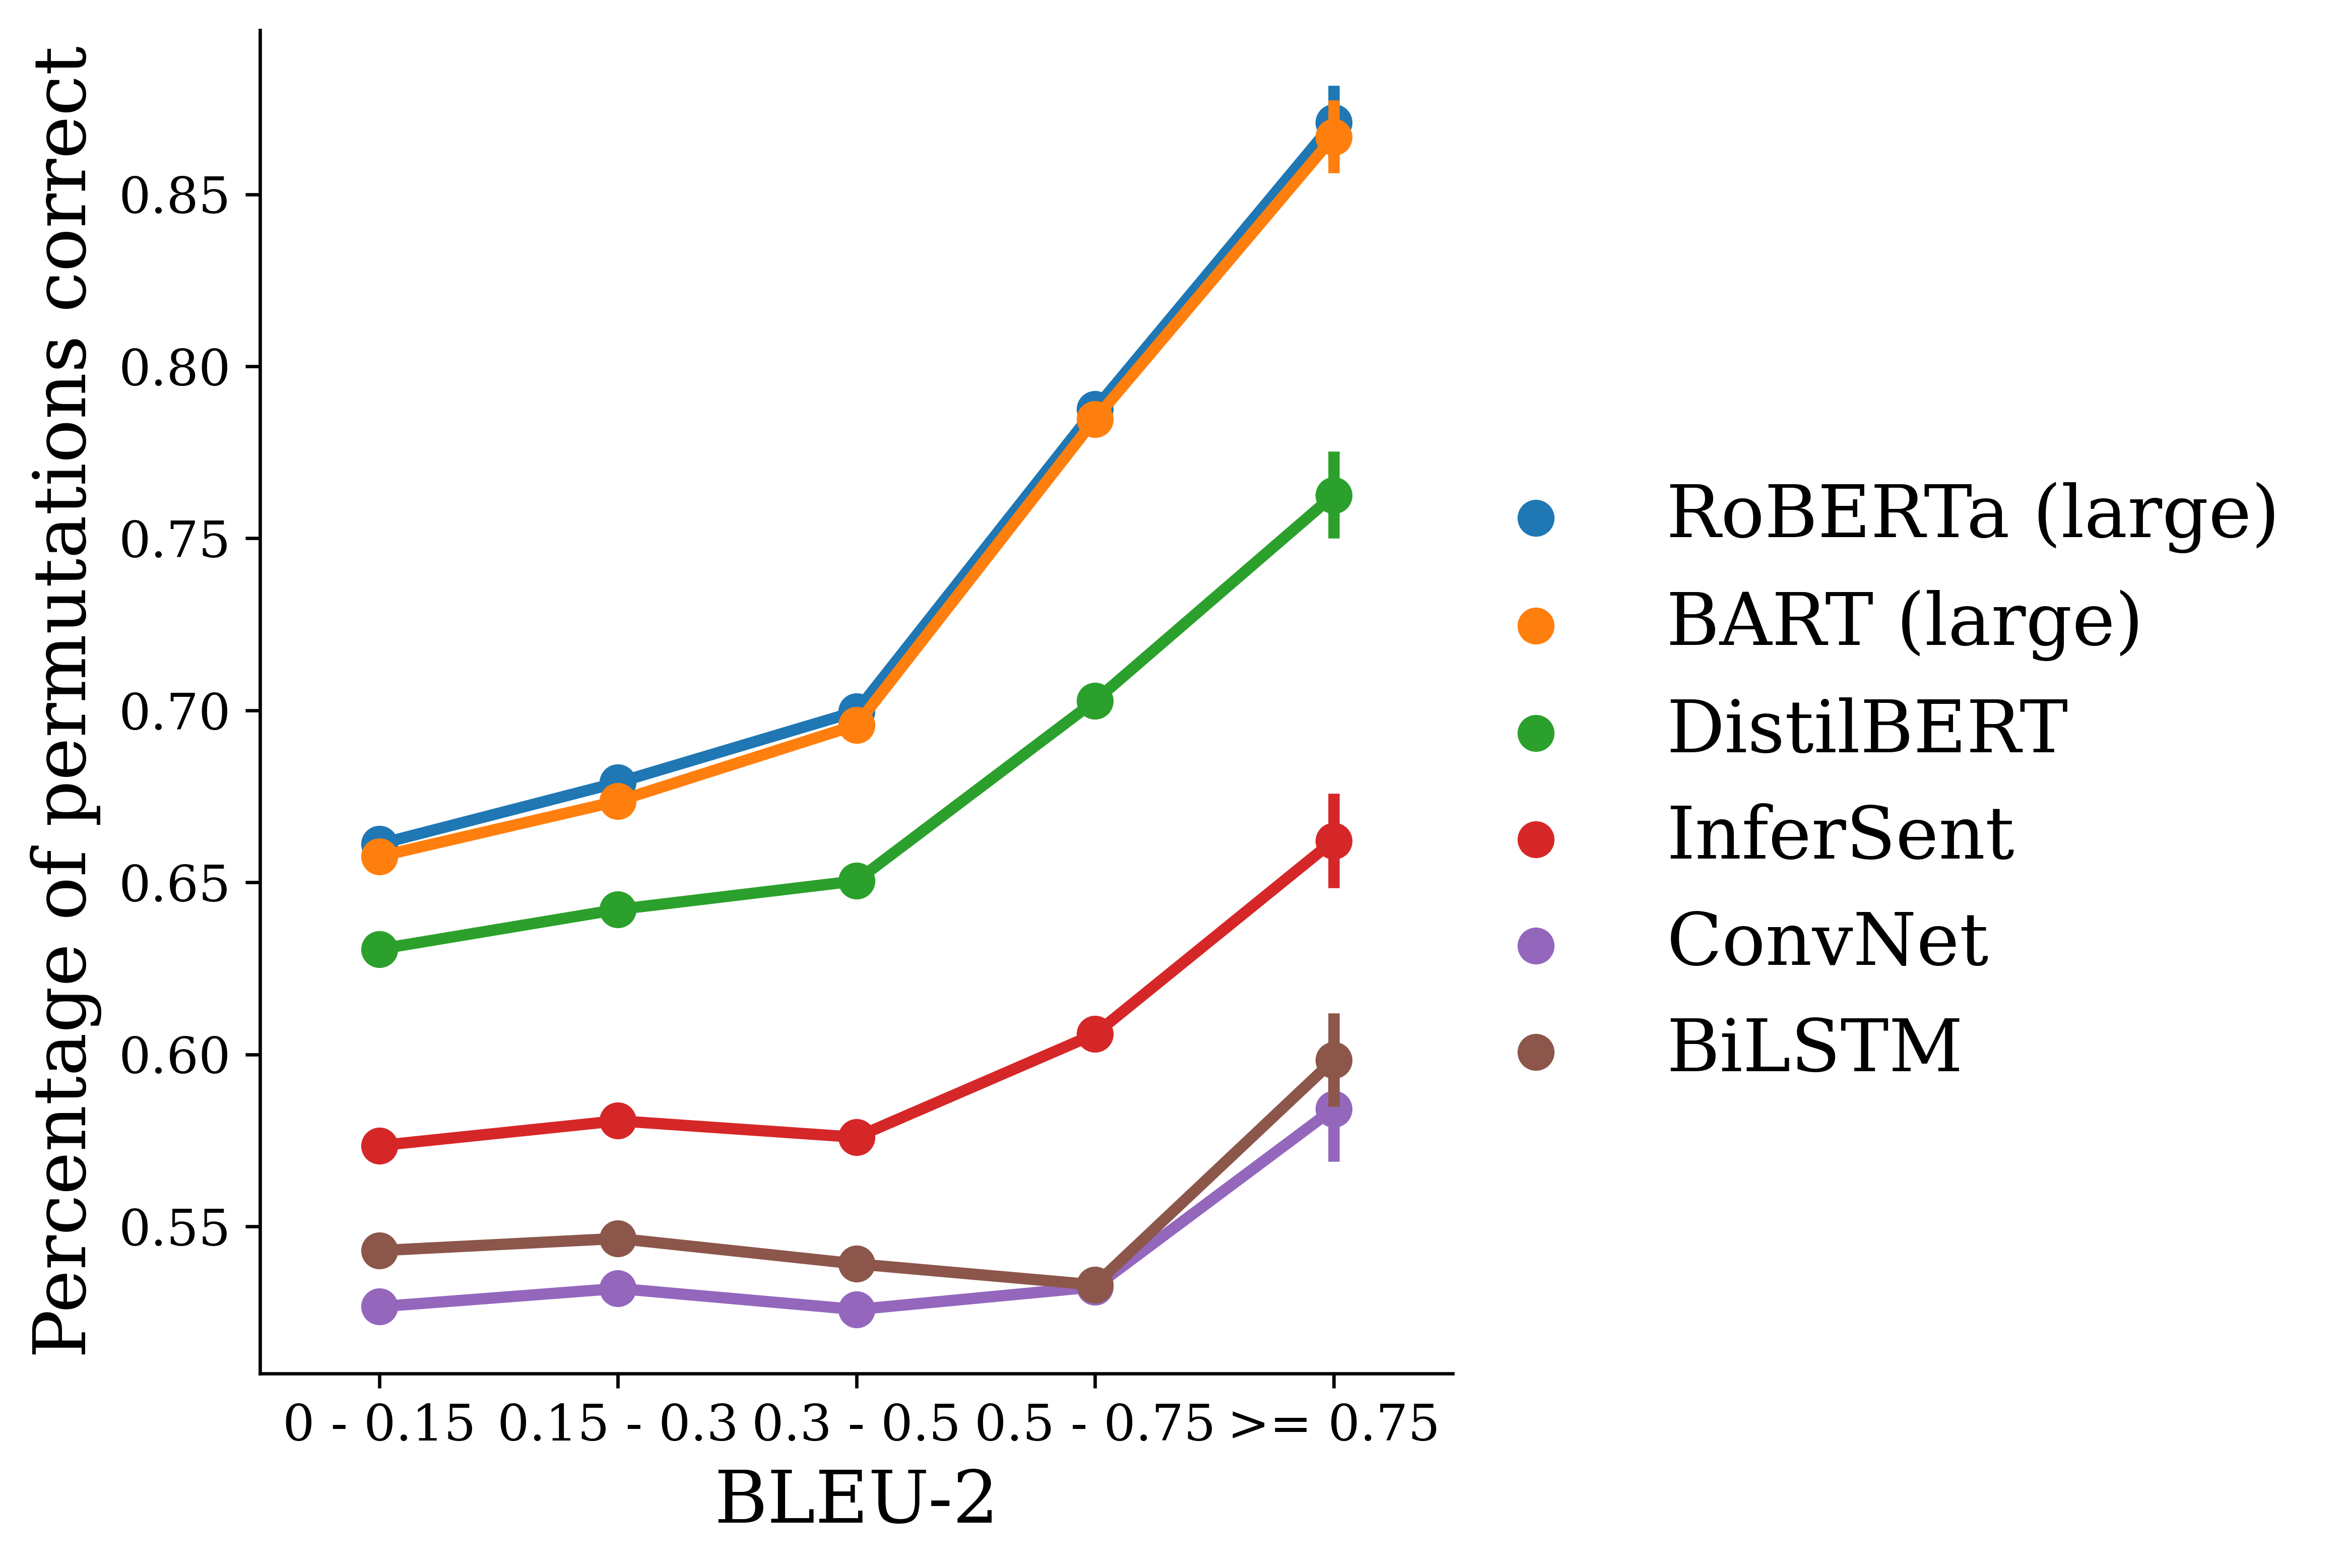
\includegraphics[width=.9\linewidth]{figs/unli/bleu_2_all.png}
\caption{BLEU-2 score versus acceptability of permuted sentences across all test datasets.}
\end{figure}

\begin{figure}[htbp]
\centering
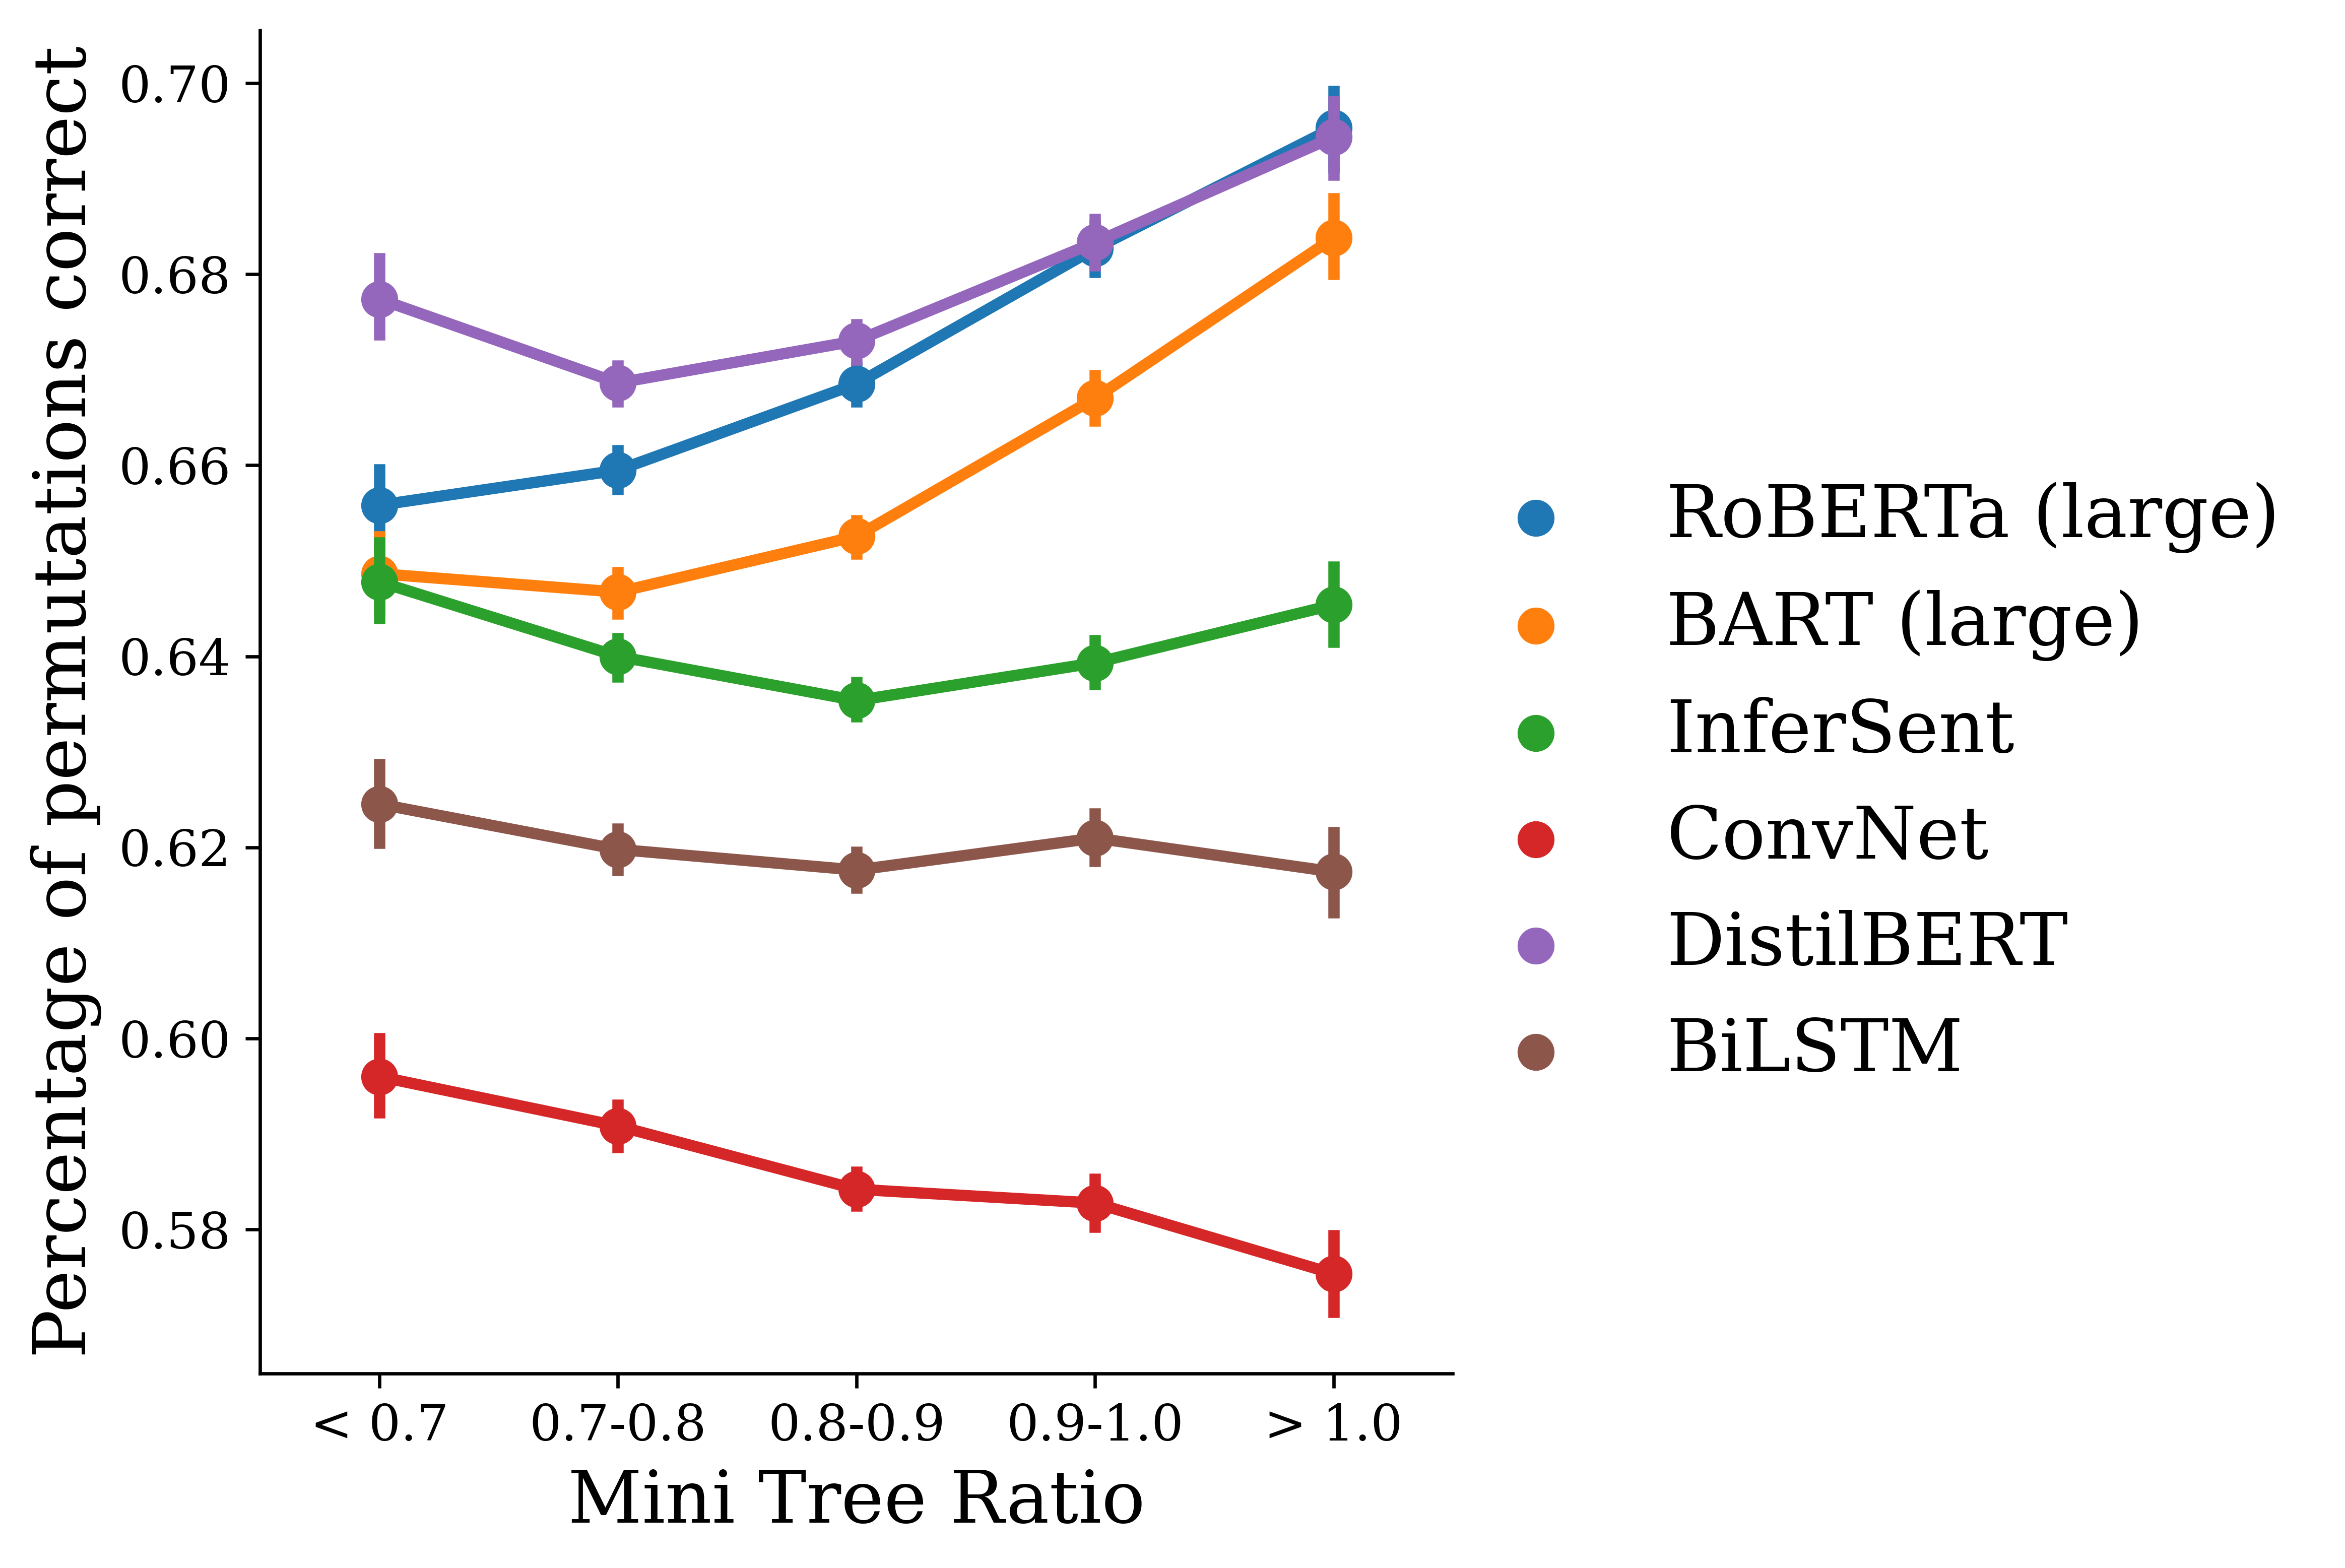
\includegraphics[width=.9\linewidth]{figs/unli/min_tree_4.png}
\caption{POS Tag Mini-Tree overlap score and percentage of permutations which the models assigned the gold label.}
\end{figure}

\begin{figure}[htbp]
\centering
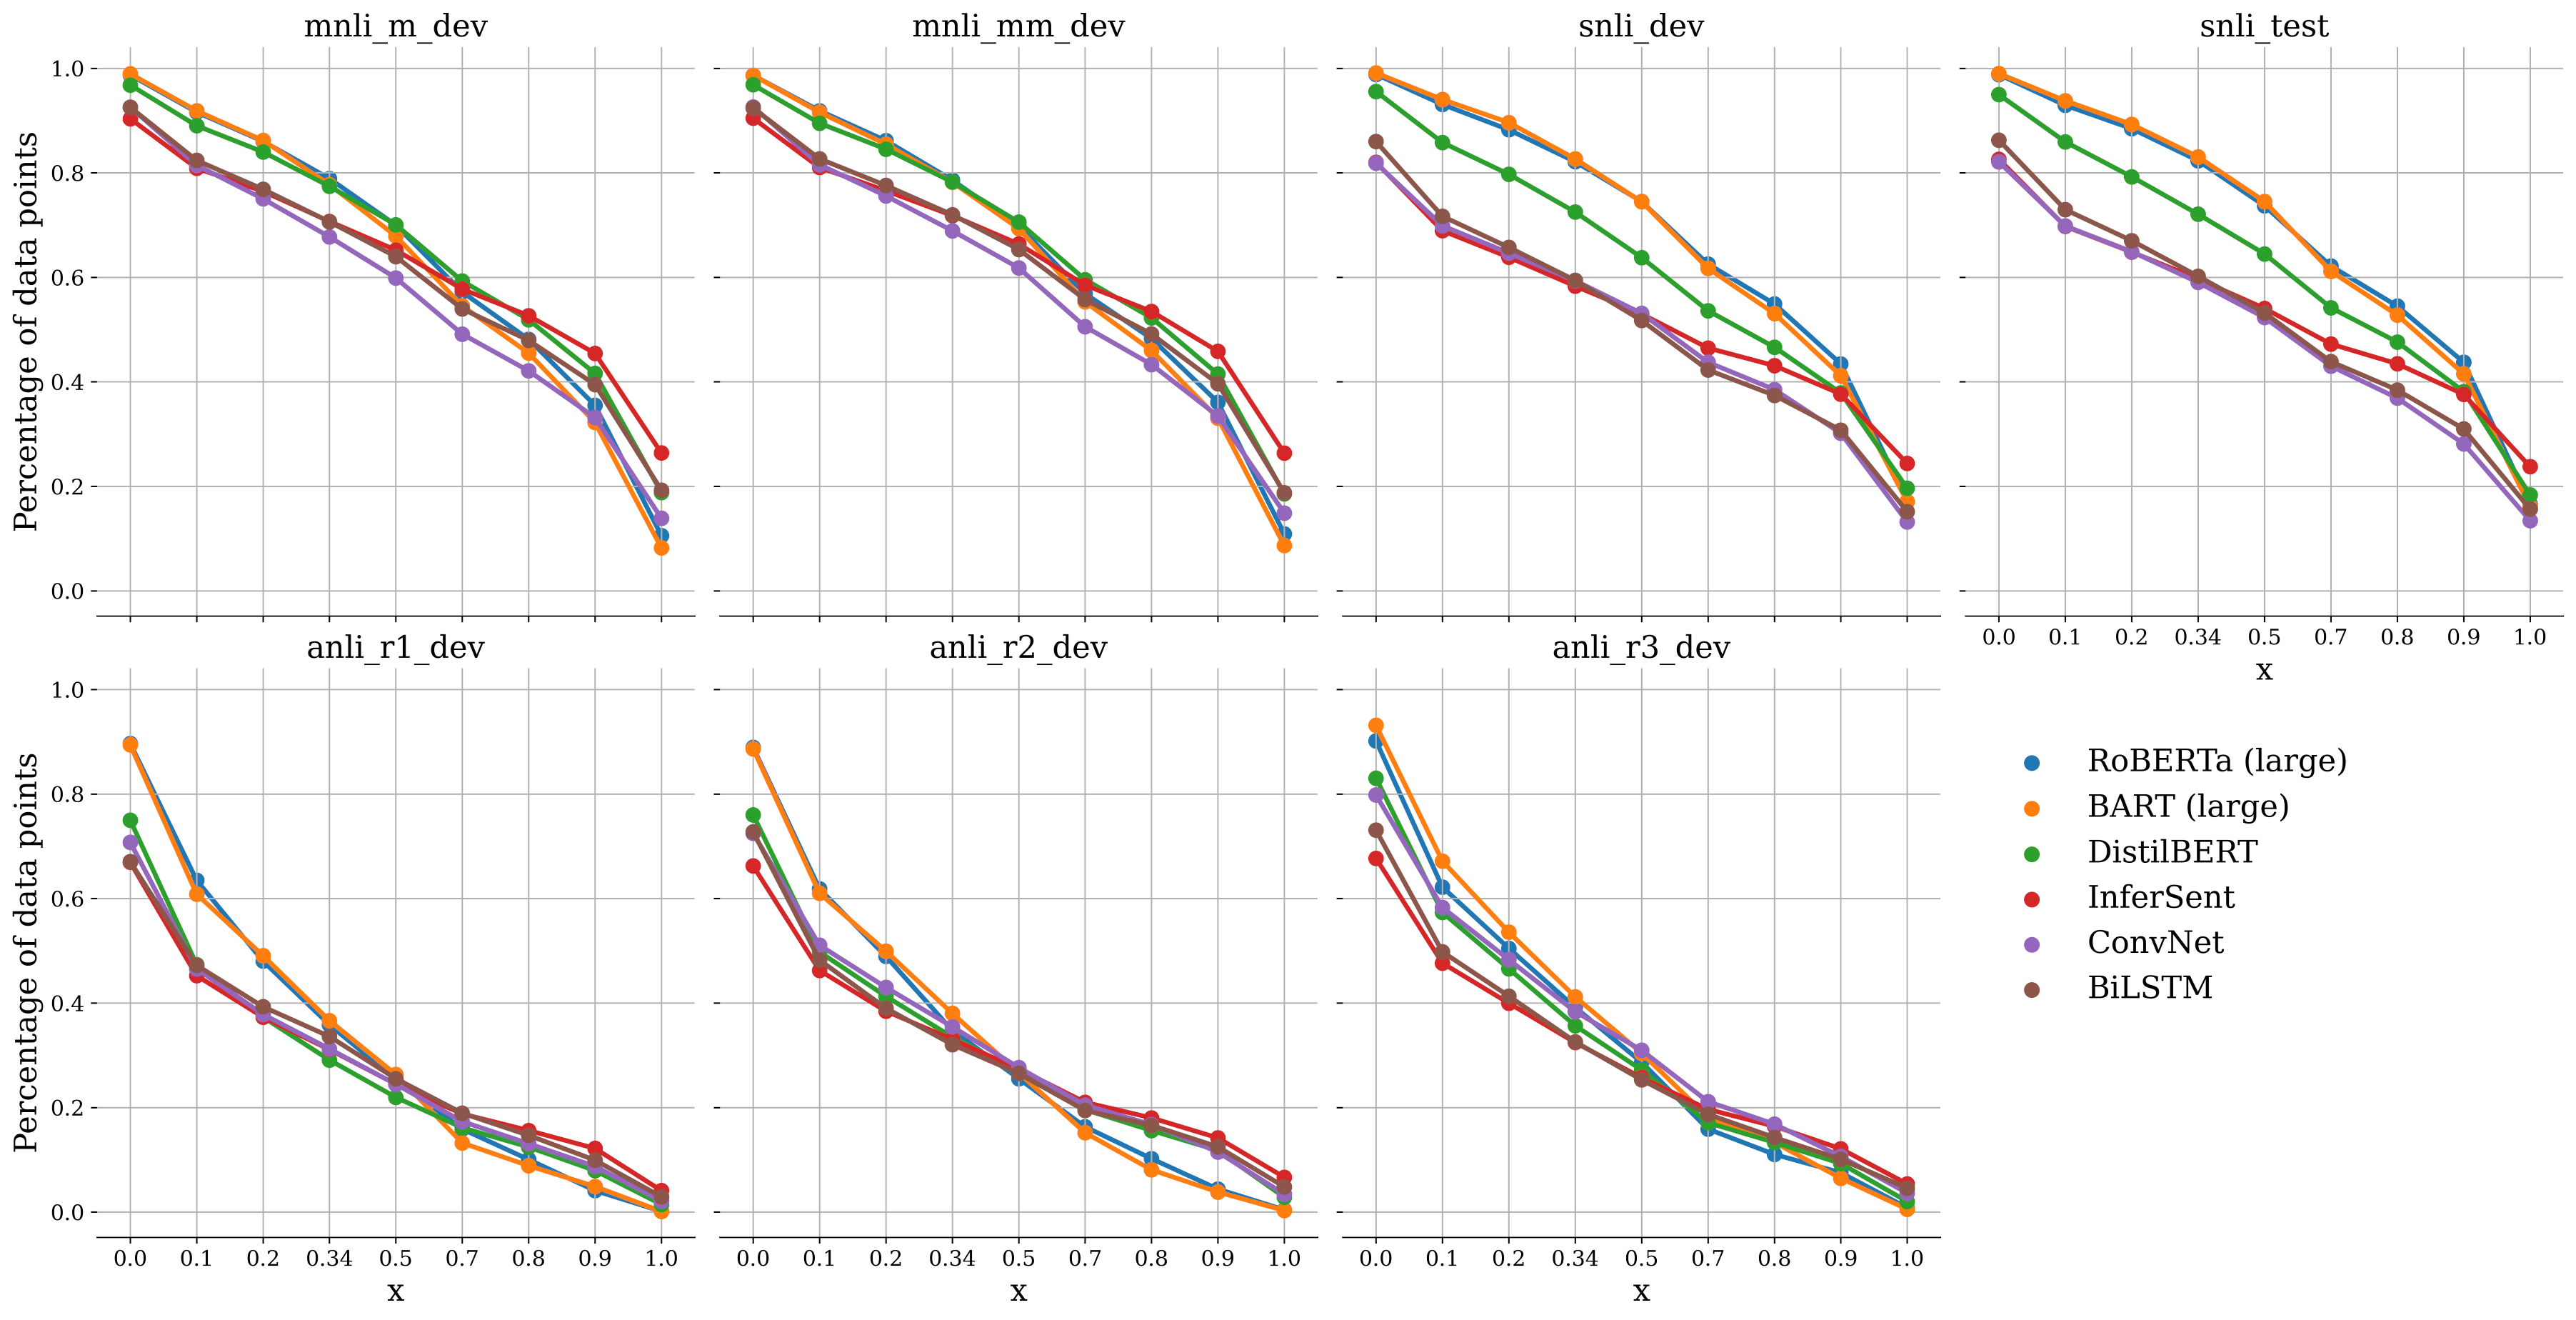
\includegraphics[width=.9\linewidth]{figs/unli/omega_threshold.png}
\caption{\(\omega_{x}\) threshold for all datasets with varying \(x\) and computing the percentage of examples that fall within the threshold.}
\end{figure}



\section{Related Work}
\label{sec:orgb553052}
\section{Discussion}
\label{sec:org6975f27}
\section{Follow-up findings in the community}
\label{sec:orgb976e8a}

\clearpage
\chapter{Probing syntax understanding through distributional hypothesis}
\label{sec:orgcdbaaa6}

Paper: \cite{sinha2021}

\section{Technical Background}
\label{sec:orgcfd03af}
\section{Dataset construction and pre-training}
\label{sec:orgc115e76}
\section{Experiments}
\label{sec:orgbbc65e2}
\subsection{Downstream reasoning tasks}
\label{sec:orge082779}

% \begin{figure}[htbp]
% \centering
% 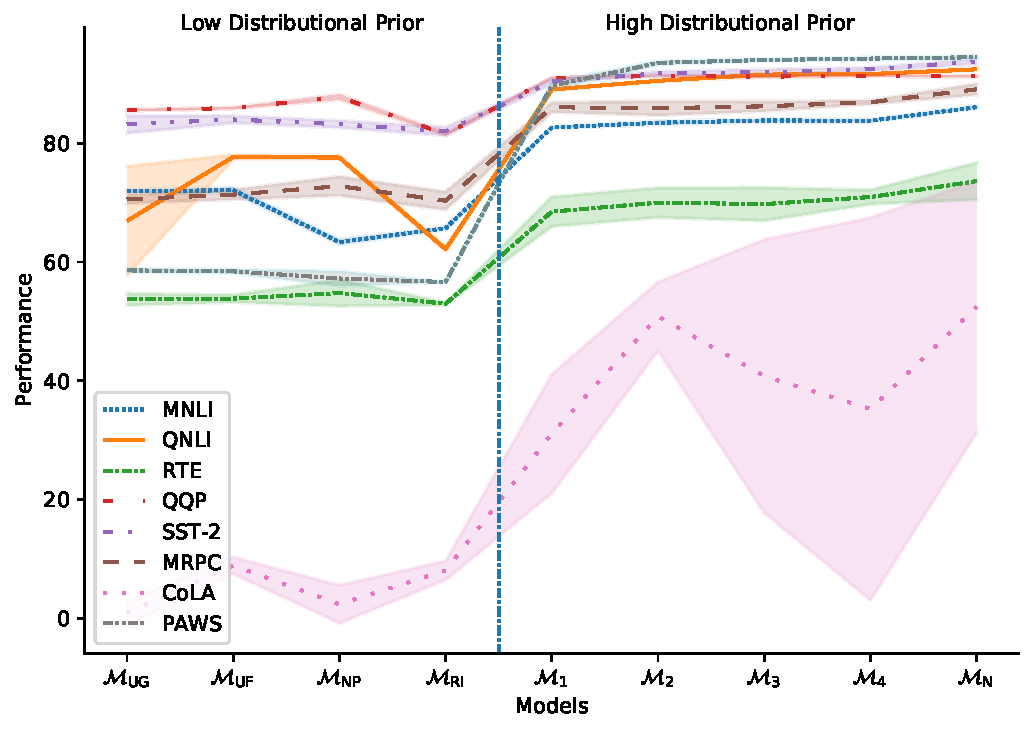
\includegraphics[width=.9\linewidth]{figs/unnat_pt/main_result_plot.pdf}
% \caption{Downstream results on scrambled pre-training.}
% \end{figure}

% \begin{figure}[htbp]
% \centering
% 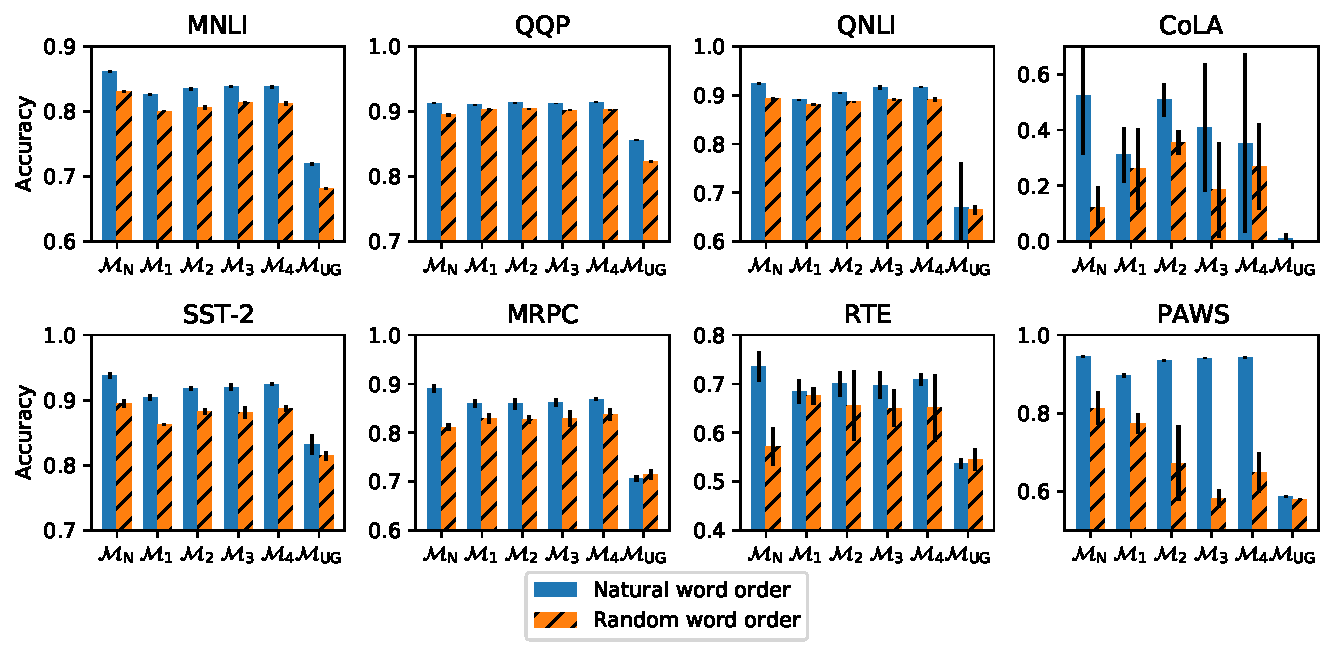
\includegraphics[width=.9\linewidth]{figs/unnat_pt/finetune_rand.pdf}
% \caption{GLUE and PAWS task dev set performance when finetuned on naturally and randomly ordered text, respectively, using pre-trained RoBERTa (base) models on different versions of BookWiki corpus.}
% \end{figure}

\subsection{Evaluating the effectiveness of probing syntax}
\label{sec:org56442b4}

% \begin{figure}[htbp]
% \centering
% 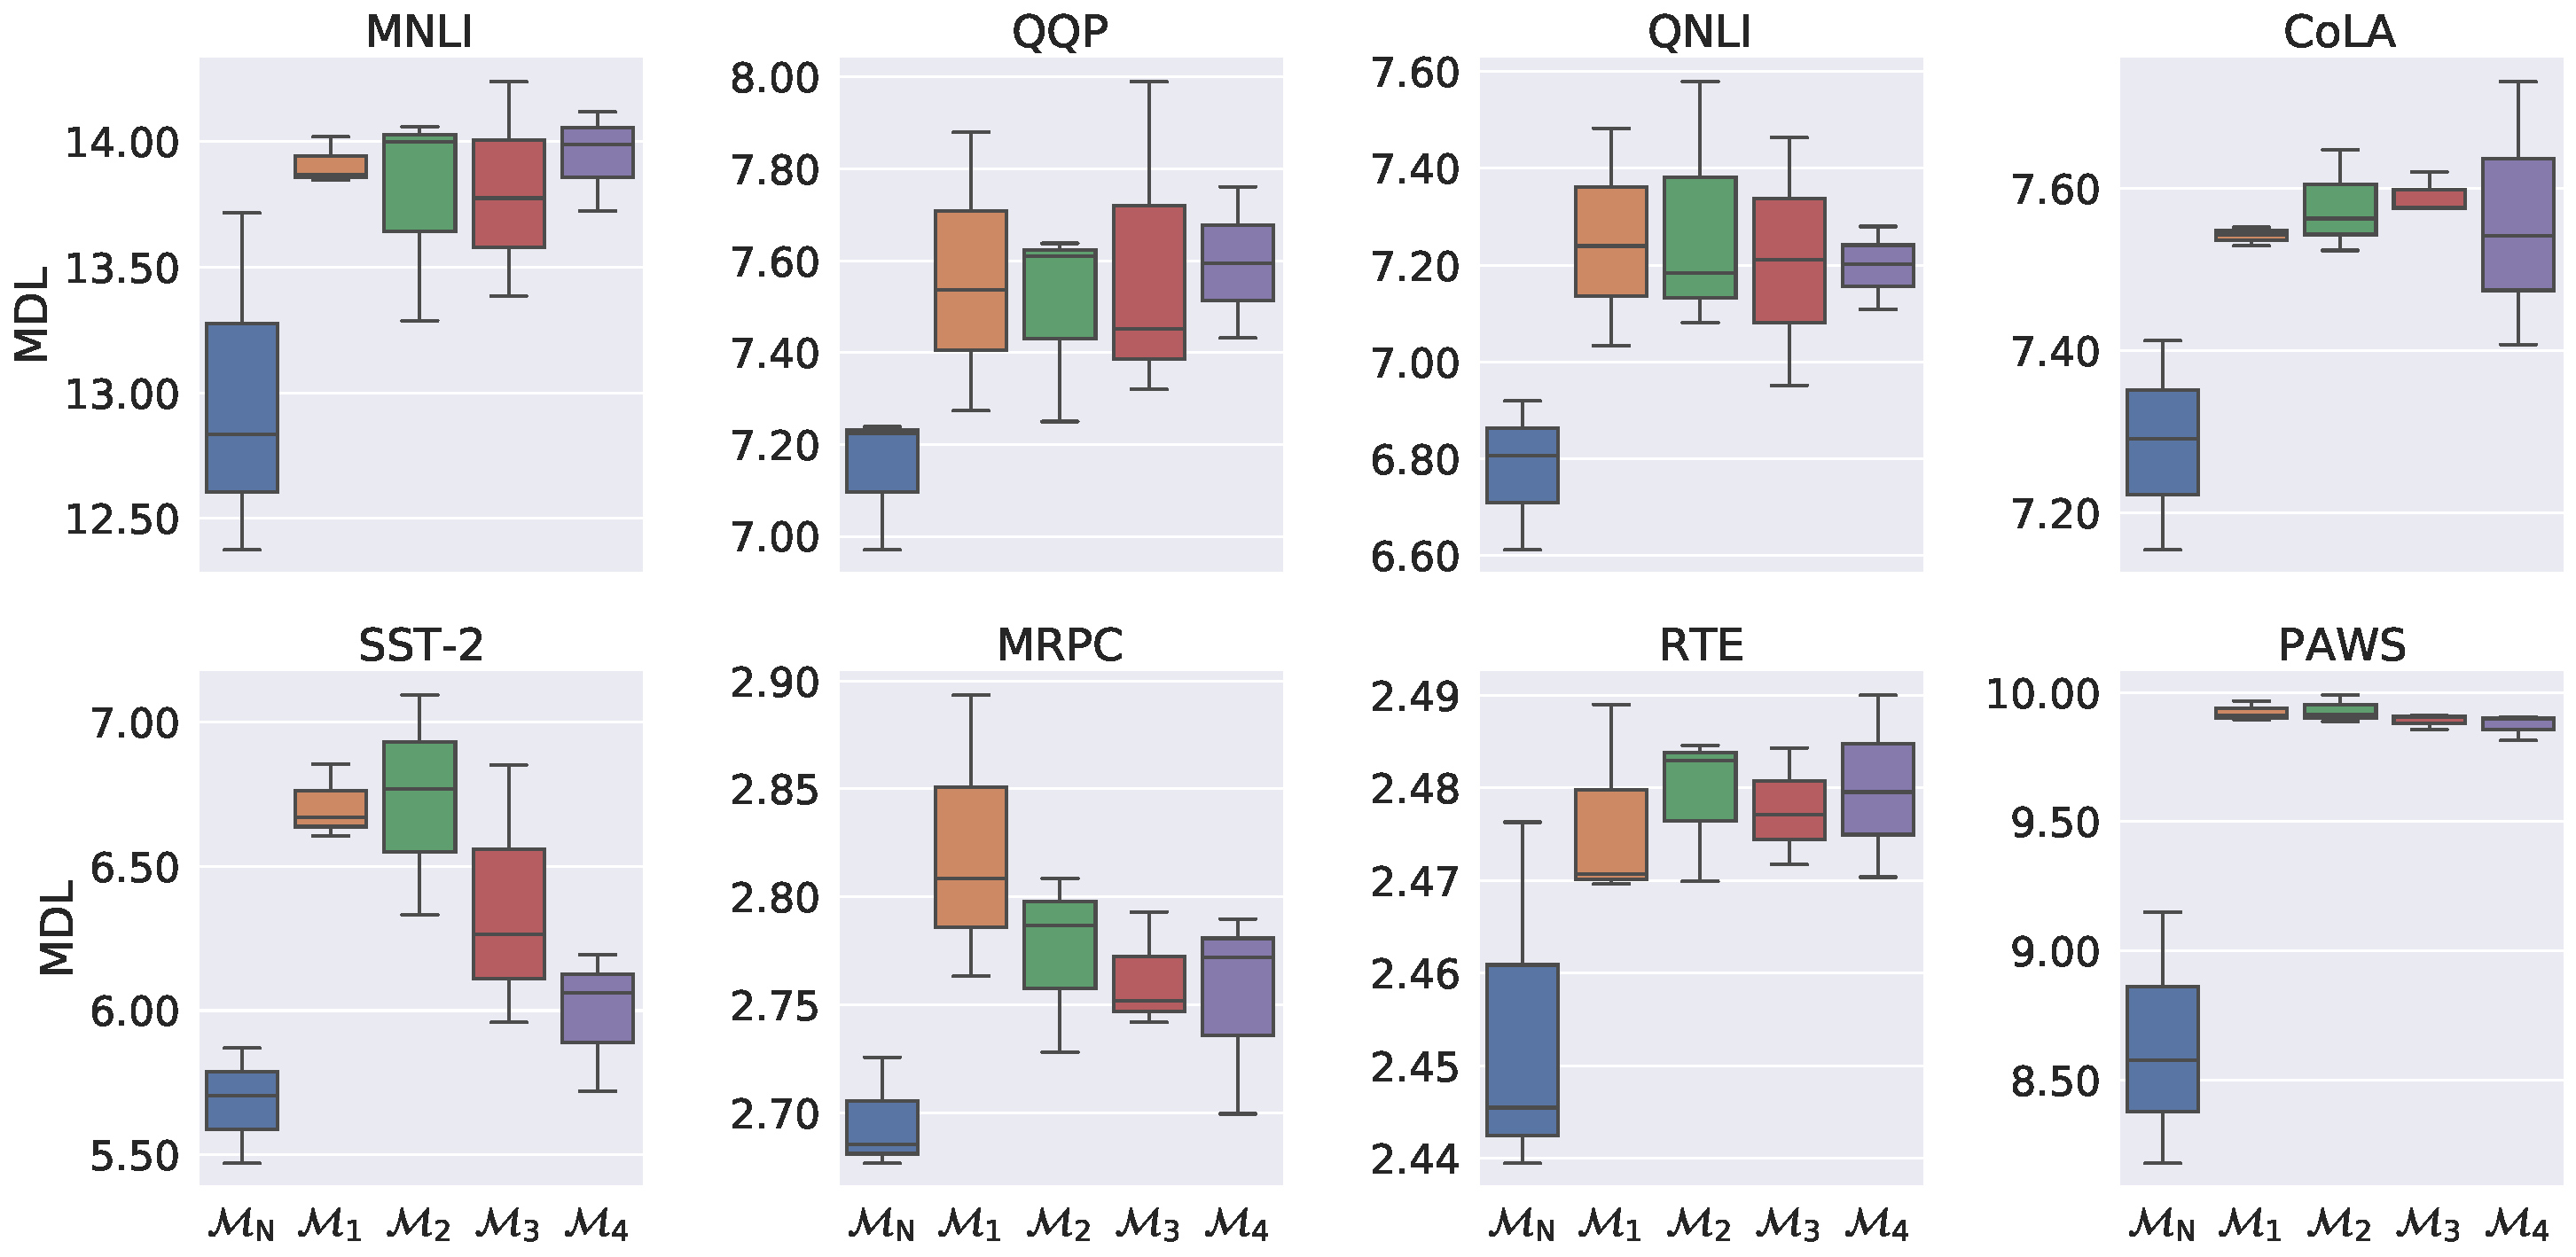
\includegraphics[width=.9\linewidth]{figs/unnat_pt/rda_mdl_ep_3.pdf}
% \caption{Risannen Data Analysis.}
% \end{figure}

\section{Related Work}
\label{sec:org0d2da32}
\section{Discussion}
\label{sec:org2941af9}
\section{Follow-up findings in the community}
\label{sec:orgde3bd47}
\clearpage
\chapter{Measuring systematic generalization by exploiting absolute positions}
\label{sec:orga46bf45}

\section{Technical Background}
\label{sec:orge8b9409}
\section{Systematic understanding of absolute position embeddings}
\label{sec:orgf8ea1d9}
\section{Related Work}
\label{sec:org05c8af6}
\section{Experiments}
\label{sec:orgc6f5de8}

% \begin{figure}[htbp]
% \centering
% 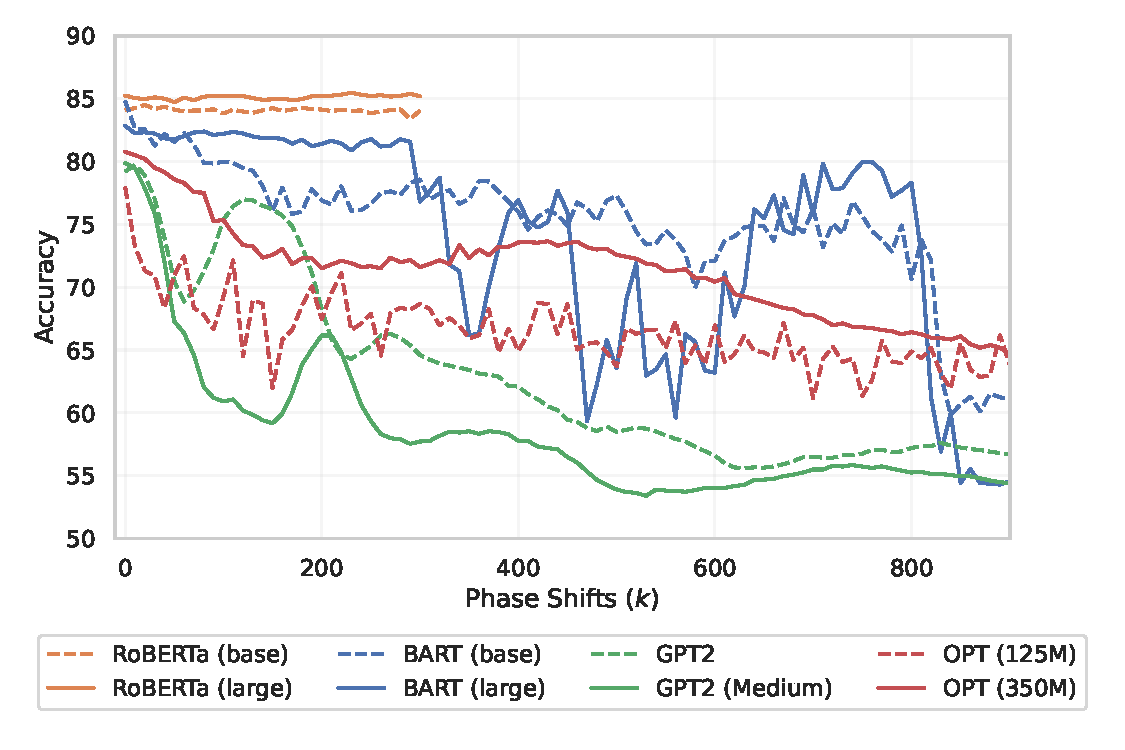
\includegraphics[width=.9\linewidth]{figs/pos_enc/acceptability_scores.pdf}
% \caption{Grammatical acceptability scores on BLiMP dataset.}
% \end{figure}

\section{Discussion}
\label{sec:orgbc43cdd}
\clearpage
\chapter{Conclusion}
\label{sec:org8fd280e}
\section{Summary}
\label{sec:org94aab9a}
\section{Limitations}
\label{sec:org217d56a}
\section{Future Work}
\label{sec:org9de237c}

\clearpage

\bibliographystyle{unsrt}
\bibliography{../../mylibrefs_new,bibfiles/unli,bibfiles/clutrr,bibfiles/pos_enc,bibfiles/unnat_pt,bibfiles/anthology}


\printglossaries

\chapter{Appendix}
\label{sec:orgd5099eb}
\section{Org mode auto save}
\label{sec:orgde5798f}
Run the following snippet to auto save and compile in org mode.

\begin{verbatim}
(defun kdm/org-save-and-export ()
(interactive)
(if (and (eq major-mode 'org-mode)
    (ido-local-file-exists-p (concat (file-name-sans-extension (buffer-name)) ".tex")))
  (org-latex-export-to-latex)))

(add-hook 'after-save-hook 'kdm/org-save-and-export)
\end{verbatim}

\section{Remove ``parts'' from report}
\label{sec:orgacef247}

\begin{verbatim}
(add-to-list 'org-latex-classes
             '("report-noparts"
               "\\documentclass[11pt]{report}"
               ("\\chapter{%s}" . "\\chapter*{%s}")
               ("\\section{%s}" . "\\section*{%s}")
               ("\\subsection{%s}" . "\\subsection*{%s}")
               ("\\subsubsection{%s}" . "\\subsubsection*{%s}")))
\end{verbatim}

\section{Add newpage before a heading}
\label{sec:org122b99a}

\begin{verbatim}
(defun org/get-headline-string-element  (headline backend info)
  (let ((prop-point (next-property-change 0 headline)))
    (if prop-point (plist-get (text-properties-at prop-point headline) :parent))))

(defun org/ensure-latex-clearpage (headline backend info)
  (when (org-export-derived-backend-p backend 'latex)
    (let ((elmnt (org/get-headline-string-element headline backend info)))
      (when (member "newpage" (org-element-property :tags elmnt))
        (concat "\\clearpage\n" headline)))))

(add-to-list 'org-export-filter-headline-functions
             'org/ensure-latex-clearpage)

\end{verbatim}

\section{Glossary and Acronym build using Latexmk}
\label{sec:org94133e2}

Add the following snippet in the file ``\textasciitilde{}/.latexmkrc'': (Source: \url{https://tex.stackexchange.com/a/44316})

\begin{verbatim}
add_cus_dep('glo', 'gls', 0, 'run_makeglossaries');
add_cus_dep('acn', 'acr', 0, 'run_makeglossaries');

sub run_makeglossaries {
    my ($base_name, $path) = fileparse( $_[0] ); #handle -outdir param by splitting path and file, ...
    pushd $path; # ... cd-ing into folder first, then running makeglossaries ...

    if ( $silent ) {
        system "makeglossaries -q '$base_name'"; #unix
        # system "makeglossaries", "-q", "$base_name"; #windows
    }
    else {
        system "makeglossaries '$base_name'"; #unix
        # system "makeglossaries", "$base_name"; #windows
    };

    popd; # ... and cd-ing back again
}

push @generated_exts, 'glo', 'gls', 'glg';
push @generated_exts, 'acn', 'acr', 'alg';
$clean_ext .= ' %R.ist %R.xdy';
\end{verbatim}
\section{Citation style buffer local}
\label{sec:org97a37f4}

\begin{verbatim}
(set (make-local-variable 'bibtex-completion-format-citation-functions)
  '((org-mode      . my/bibtex-completion-format-citation-org-default-cite)))
\end{verbatim}
\section{Org latex compiler options}
\label{sec:orgc7e24c0}

\begin{verbatim}
(setq org-latex-pdf-process (list "latexmk -f -pdf -%latex -interaction=nonstopmode -output-directory=%o %f"))
\end{verbatim}

Original value

\begin{verbatim}
(setq org-latex-pdf-process (list "latexmk -f -pdf %f"))
\end{verbatim}

Let us try Fast compile \url{https://gist.github.com/yig/ba124dfbc8f63762f222}.

\begin{verbatim}
(setq org-latex-pdf-process (list "latexmk-fast %f"))
\end{verbatim}

\begin{itemize}
\item Doesn't seem to work from Emacs.
\item I need to change the save function to only export in tex. Then, have a separate process run latexmk.
\item Using the python package \texttt{when-changed} to watch the thesis.tex file for change.
\item Usage:
\end{itemize}

\begin{verbatim}
when-changed thesis.tex latexmk -f -pdf -interaction=nonstopmode -output-directory=%o thesis.tex
\end{verbatim}

\begin{itemize}
\item The pdf does not update. It seems to but not always? No it does. For some reason, compilation takes ages.
\item Works with \texttt{when-changed}!
\end{itemize}
\end{document}
